%; whizzy chapter
% -initex iniptex -latex platex -format platex -bibtex jbibtex -fmt fmt
% 以上 whizzytex を使用する場合の設定。

%     Kansai Debian Meeting resources
%     Copyright (C) 2007 Takaya Yamashita
%     Thank you for Tokyo Debian Meeting resources

%     This program is free software; you can redistribute it and/or modify
%     it under the terms of the GNU General Public License as published by
%     the Free Software Foundation; either version 2 of the License, or
%     (at your option) any later version.

%     This program is distributed in the hope that it will be useful,
%     but WITHOUT ANY WARRANTY; without even the implied warranty of
%     MERCHANTABILITY or FITNESS FOR A PARTICULAR PURPOSE.  See the
%     GNU General Public License for more details.

%     You should have received a copy of the GNU General Public License
%     along with this program; if not, write to the Free Software
%     Foundation, Inc., 51 Franklin St, Fifth Floor, Boston, MA  02110-1301 USA

%  preview (shell-command (concat "evince " (replace-regexp-in-string "tex$" "pdf"(buffer-file-name)) "&"))
% 画像ファイルを処理するためにはebbを利用してboundingboxを作成。
%(shell-command "cd image200708; ebb *.png")

%%ここからヘッダ開始。

\documentclass[mingoth,a4paper]{jsarticle}
\usepackage{kansaimonthlyreport}
\usepackage[dvips]{xy}
\usepackage{ulem}

% 日付を定義する、毎月変わります。
\newcommand{\debmtgyear}{2018}
\newcommand{\debmtgdate}{22}
\newcommand{\debmtgmonth}{4}
\newcommand{\debmtgnumber}{134}

\def\fixme#1{{\color{red}{#1}}}

\begin{document}

\begin{titlepage}

% 毎月変更する部分、本文の末尾も修正することをわすれずに

 第\debmtgnumber{}回 関西 Debian 勉強会資料

\vspace{2cm}

\begin{center}
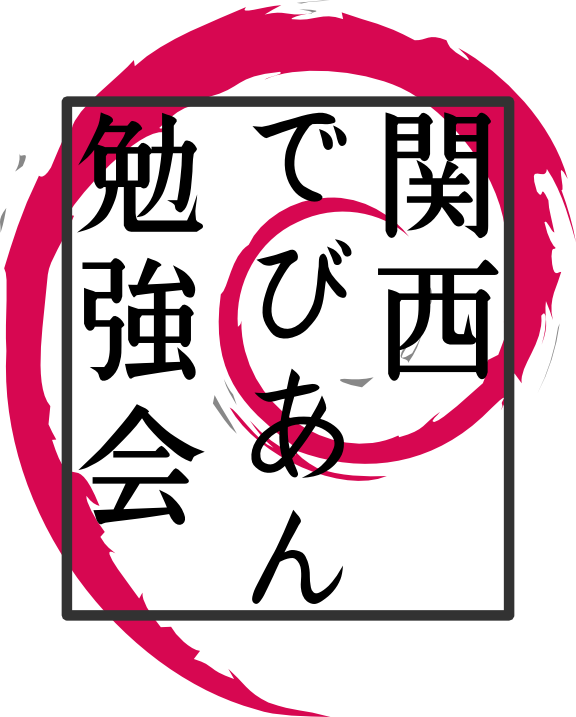
\includegraphics{image200802/kansaidebianlogo.png}
\end{center}

\begin{flushright}
\hfill{}関西 Debian 勉強会担当者 佐々木・倉敷・のがた・かわだ・おおつき \\
\hfill{}\debmtgyear{}年\debmtgmonth{}月\debmtgdate{}日
\end{flushright}

\thispagestyle{empty}
\end{titlepage}

\dancersection{最近のDebian関係のイベント報告}{Debian JP}

\subsection{第133回関西Debian勉強会}
3 月 25 日に福島区民センターで開催されました。発表は川江 浩さんによる「我が家の仮想ネットワーク」でした。

\subsection{第162回東京エリアDebian勉強会}
4 月 21 日に朝日ネットさんで開催されました。発表は行われず hack time を中心とした集まりでした。

\dancersection{最近のDebian News}{Debian JP}

\subsection{2018/Mar/16th Debian Conference 2018 registration 開始}
			call for parapers は 2018/June/18th https://debconf18.debconf.org/cfp/
\subsection{Debian Policy v4.1.4.1 がリリース}
	\begin{itemize}
		\item 2018/Apr/07th
		\item \url{https://www.debian.org/doc/debian-policy/}
		\item 差分を確認する get-orig-source が廃止に、かわりに uscan と debian/watch を使うようにとのこと
		\item \url{https://lists.debian.org/debian-devel/2018/04/msg00081.html}
	\end{itemize}
\subsection{kFreeBSD と (Hurd) の buildd がパッケージ化}
	\begin{itemize}
		\item sid でパッケージ化されたとのこと
		\item kFreeBSD 用のパッチをどしどし書いてくださいとのこと
		\item \url{https://lists.debian.org/debian-devel/2018/04/msg00492.html}
	\end{itemize}
%\subsection{m68k 科学計算系のパッケージは直さなくてもいいのでは?}
%	\begin{itemize}
%	\item R 言語のビルドが m68k qemu のバグが原因で失敗した。	実際に使っているユーザーもいないだろうし、	科学計算系のパッケージがビルドに失敗しても直さなくていいのでは? との提案でした。
%	\item m68k ユーザーら反発
%	\item m68k ユーザー曰く「科学計算系のパッケージの品質が悪いかからだ。」とのこと
%	\item \url{https://lists.debian.org/debian-devel/2018/03/msg00448.html}
%	\end{itemize}

\dancersection{事前課題}{関西Debian勉強会}

\begin{itemize}
	\item 以下の資料に目を通しておいて下さい。
	\begin{itemize}
		\item https://wiki.debian.org/sbuild
		\item https://wiki.debian.org/LXC
	\end{itemize}
	\item (推奨)会場で利用できるネットワーク環境をご用意ください。
\end{itemize}

参加者の皆さんは以下の通りです:
\begin{prework}{Katsuki Kobayashi}
\end{prework}

\begin{prework}{uwabami}
\end{prework}
 
\begin{prework}{tomabu}
\end{prework}
 
\begin{prework}{znz}
\end{prework}
 
\begin{prework}{ipv6waterstar}
\end{prework}
 
\begin{prework}{t3rkwd}
\end{prework}
 
\begin{prework}{yosuke\_san}
\end{prework}
 
\begin{prework}{ItSANgo}
\end{prework}
 
\begin{prework}{榎真治} 
\end{prework}

\dancersection{最近のDebianパッケージ作成環境 - git-buildpackage, sbuild, autopkgtest を例に -}{佐々木 洋平}

\clearpage

\dancersection{開催の予定}{}

\begin{itemize}
	\item {5 月 27 日 福島区民センター 304 号室} 
	\item {6 月 24 日 福島区民センター 304 号室} 
	\item {8 月 26 日 福島区民センター 304 号室} 
	\item {9 月 23 日 福島区民センター 304 号室} 
\end{itemize}

\vspace{\fill}
本資料は GPL v 2.0 のライセンスで公開いたします。

\clearpage

%
% 冊子にするために、4の倍数にする必要がある。
% そのための調整

\mbox{}\newpage
\mbox{}\newpage

\printindex
%\cleartooddpage

 \begin{minipage}[b]{0.2\hsize}
  \rotatebox{90}{\fontsize{80}{80} {\gt 関西 Debian 勉強会} }
 \end{minipage}
 \begin{minipage}[b]{0.8\hsize}

 \vspace*{15cm}
 \rule{\hsize}{1mm}
 \vspace{2mm}
 
\includegraphics[width=2cm]{image200502/openlogo-nd.eps}
 \noindent \Large \bfseries{Debian 勉強会資料}\\ \\
 \noindent \normalfont \debmtgyear{}年\debmtgmonth{}月\debmtgdate{}日 \hspace{5mm}  初版第1刷発行\\
 \noindent \normalfont 関西 Debian 勉強会 (編集・印刷・発行)\\
 \rule{\hsize}{1mm}
 \end{minipage}

\end{document}




